\section{Route 1: Fahrradtunnel Universitäten}
Folgende Route schlagen wir als Hauptverbindung im Grazer Osten in Tunnelform vor:

\begin{itemize}
    \item Schulzentrum St. Peter
    \item Neue Technik
    \item Alte Technik
    \item Lichtenfelsgasse
    \item KFU Hauptgebäude (Kreuzung mit Route 2)
    \item Kreuzschwestern-Park
    \item Wirtschaftskammer/Campus02
\end{itemize}

\begin{figure}
    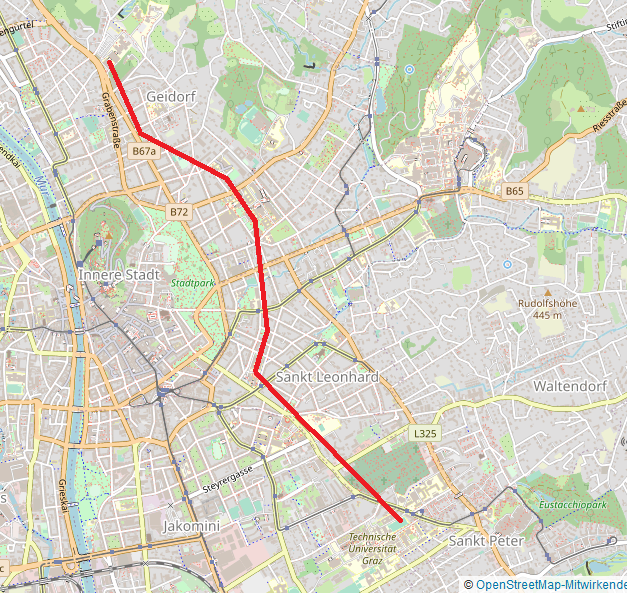
\includegraphics[width=0.8\textwidth]{main/bike/tunnel/uni/linie1}
    \centering
    \caption[Verlauf Linie 1]{Verlauf der Linie 1 zwischen den Zufahrten}
\end{figure}

Zwischen den einzelnen Universitäten findet oft besonders reger Radverkehr statt, und auf dieser Achse ist aufgrund der Bauweise der Stadt oft besonders wenig Platz für Radinfrastruktur.

Dieser Tunnel stellt eine Achse Nord-Süd dar und ist mit einer Kreuzung sowohl mit dem Stadtzentrum als auch dem Landeskrankenhaus verbunden.

\subsection{Zufahrt Schulzentrum St. Peter}
Die Zufahrt \index{Schulzentrum St. Peter} soll (vorläufig) der südlichste Punkt der Linie 1 sein und damit sowohl selbst ein großes Einzugsgebiet als auch eine gute Anbindung an den weiteren Verkehr haben. Beides ist gegeben; nicht umsonst ist die Haltestelle Schulzentrum St. Peter schon aktuell ein wichtiger Verkehrsknotenpunkt für den öffentlichen Verkehr.

Die Zufahrt soll direkt an der Straßenbahnhaltestelle Schulzentrum St. Peter liegen.

\begin{figure}
    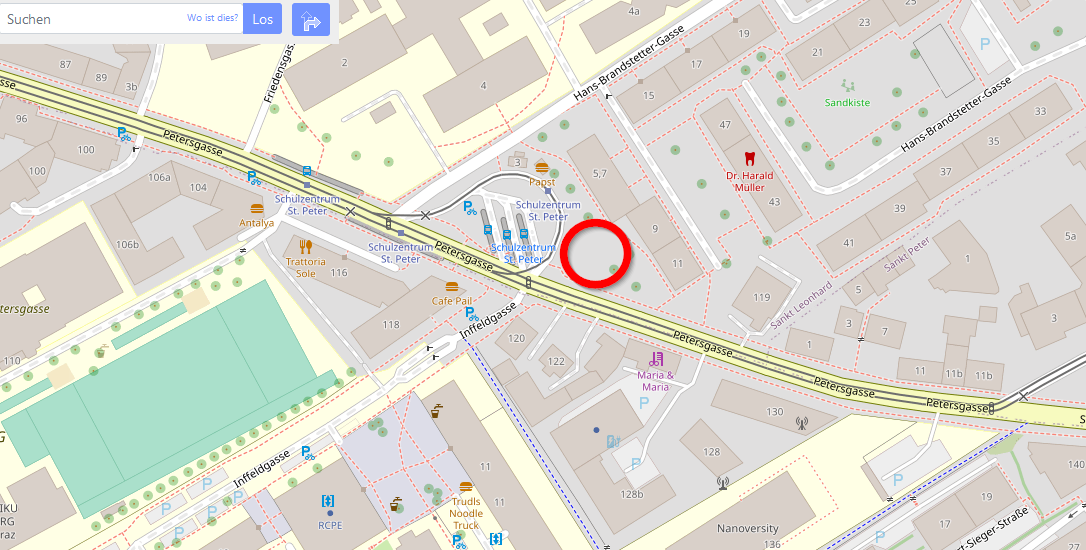
\includegraphics[width=0.8\textwidth]{main/bike/tunnel/uni/zufahrt_inffeld}
    \centering
    \caption[Zufhart St. Peter Schulzentrum]{Vorgeschlagener Ort der Zufahrt in den Tunnel der Linie 1}
\end{figure}

Die Zufahrt selbst wird einen Teil des Grünbereichs neben der Haltestelle auffressen.

Durch diese Zufahrt wird das gesamte Schulzentrum erschlossen, zu dem unter anderem die \index{Berufsschule St. Peter}, der \index{Campus Inffeldgasse} der Technischen Universität Graz, das \index{BRG Petersgasse} und das \index{WIKU BRG Graz} gehören.

Damit die Zufahrt besser an den Verkehr angebunden ist, sind hier weitere Maßnahmen nötig:

\paragraph{Fahrradgarage St. Peter Schulzentrum}
Direkt im Bereich der Zufahrt sollte eine Parkgarage für Fahrräder unterirdisch errichtet werden. Diese Garage kann sowohl dazu dienen, das Fahrrad dort abzustellen, während man eine der Ausbildungsstätten besucht, als auch als Park-and-Ride-Lösung für Personen, die von hier aus mit dem Bus oder der Straßenbahn weiterfahren wollen.

\paragraph{Anschluss Berufsschule}
Es soll eine Möglichkeit geschaffen werden, von der Zufahrt direkt auf das Gelände der Berufsschule St. Peter zu gelangen. Dafür ist die Errichtung eines weiteren (kurzen) Radweges nötig, der auch eine sichere Querung der \index{Hans-Brandstetter-Gasse} erlaubt.

\paragraph{Straßenquerung Petersgasse}
Ein signifikanter Teil der Benutzer der Zufahrt werden aus der \index{Inffeldgasse} kommen bzw. in die Inffeldgasse weiterfahren wollen, um einerseits den Campus Inffeldgasse der Technischen Universität Graz zu erreichen, als auch den Anschluss an die Radroute \index{Neufeldweg}, die am westlichen Ende der Inffeldgasse ihren Anfang nimmt. Dafür ist eine sichere Querung der \index{Petersgasse} nötig. Da die Petersgasse eine wichtige Route für den motorisierten Individualverkehr ist, gibt es hier inhärentes Konfliktpotential.

\paragraph{Alternative: Zwei Ausfahrten}
Um das Konfliktpotential in der Petersgasse zu umgehen, wäre es auch denkbar, eine Unterführung unter der Straße anzubieten und eine zweite Ausfahrt am Anfang der Inffeldgasse zu bauen, sodass die Zufahrt St. Peter Schulzentrum letztlich aus zwei unterschiedlichen Zufahrten besteht. Das hat natürlich den Nachteil höherer Kosten, löst aber den Konflikt in der Petersgasse komplett auf.

\subsection{Zufahrt Neue Technik}
Die nächste Zufahrt soll im Bereich der \index{Neuen Technik} liegen. Einerseits ist der Radpendelverkehr zwischen Inffeldgasse und Neuer Technik traditionell immer sehr hoch, andererseits gibt es dafür oberirdisch keine vernünftige Möglichkeit, weswegen es zu zahlreichen Konflikten zwischen Autofahrern und Radfahrern auf der \index{Petersgasse} kommt.

\begin{figure}
    \centering
    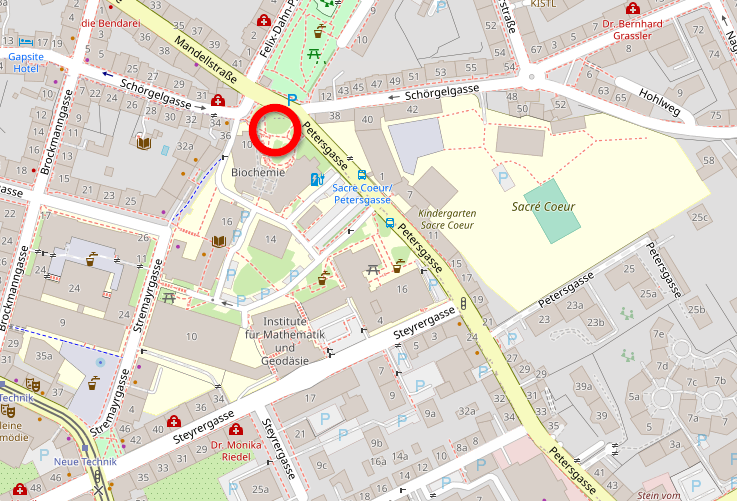
\includegraphics[width=0.8\textwidth]{main/bike/tunnel/uni/zufahrt_neue_technik}
    \caption[Zufahrt Neue Technik]{Ort der Zufahrt Neue Technik auf dem Vorplatz der Biochemie}
\end{figure}

\paragraph{Anschluss}
Von hier aus ist ein guter Anschluss an das weitere Radwegenetz gegeben. Über die \index{Schörgelgasse} gelangt man direkt zum \index{Dietrichsteinplatz} und über den anschließenden Radweg in die \index{Koperinikusgasse}. Auf der anderen Straßenseite befindet sich mit dem \index{Sacré Coeur} eine weitere größere Schule.

\paragraph{Fahrradgarage}
An dieser Zufahrt bietet sich eien unterirdische Fahrradgarage sehr an, da hier die Stellplätze an der Oberfläche begrenzt sind. Sowohl das Geländer der Neuen Technik als auch des Sacré Coeur bieten Stellmöglichkeiten an, die sind jeweils aber sehr begrenzt.

\paragraph{Umgestaltung der Kreuzung Schörgelgasse/Petersgasse/Mandellstraße}
\begin{figure}
    \centering
    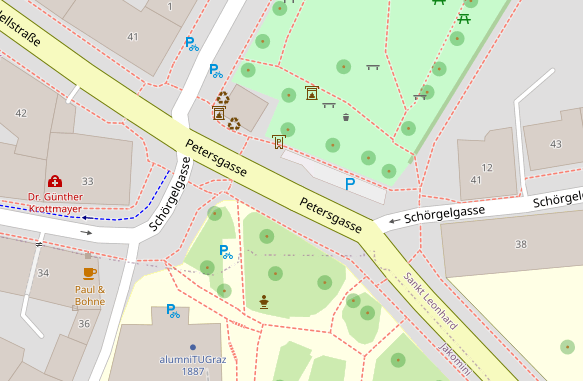
\includegraphics[width=0.6\textwidth]{main/bike/tunnel/uni/kreuzung1}
    \caption[Petersgasse/Mandellstraße mit Kreuzung Schörgelgasse]{Die Petersgasse mit den Einmündungen der Schörgelgasse ist aktuell bereits ein unübersichtlicher Bereich.}
\end{figure}

Die Mandellstraße geht bei der ersten Einmündung der Schörgelgasse in die Petersgasse über. Diese Kreuzung ist bisher schon recht unübersichtlich, da hier zahlreiche unterschiedliche Verkehrsteilnehmer in unterschiedliche Richtungen abbiegen. Es gibt einen Zebra-Streifen, mehrere Fahrradspuren und die zwei sehr nah beieinanderliegenden Kreuzungen Felix-Dahn-Platz/Mandellstraße/Petersgasse/Schörgelgasse und Petersgasse/Schörgelgasse.

\paragraph{Option: Unterirdische Querung der Petersgasse}
Als Option wäre eine unterirdische Querung der Petersgasse denkbar, evtl. ein direkter Zugang zum Sacré Coeur von der Fahrradgarage aus, sodass hier die Querung der Petersgasse nicht mehr nötig ist, wenn man von der Zufahrt zum Sacré Coeur möchte.

\subsection{Zufahrt Alte Technik}
Ein weiterer häufig benutzter Weg, der an der Oberfläche über kaum Fahrradinfrastruktur verfügt, ist die Verbindung zwischen der Neuen Technik und der \index{Alten Technik}.

\paragraph{Ort der Zufahrt}
\begin{figure}
    \centering
    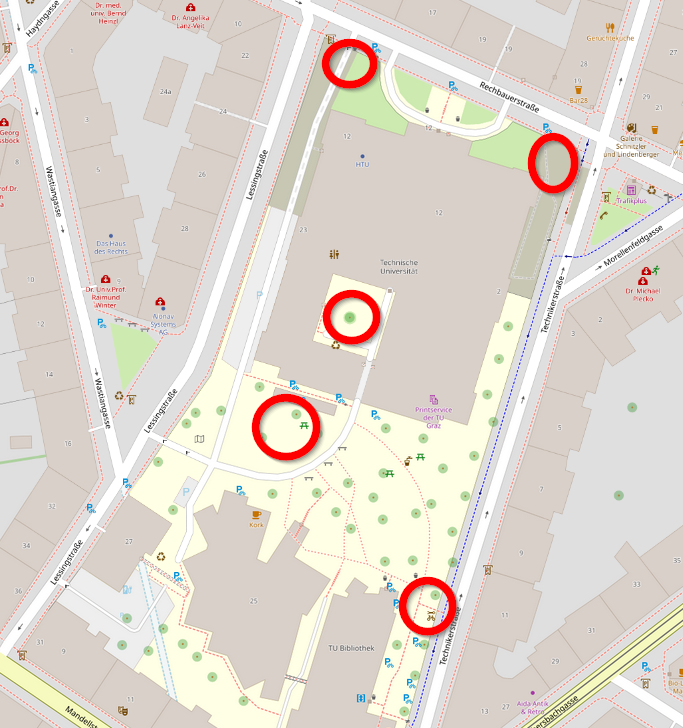
\includegraphics[width=0.6\textwidth]{main/bike/tunnel/uni/zufahrt_alte_technik}
    \caption[Zufahrten Alte Technik]{Es gibt hier mehrere Möglichkeiten für die Zufahrt zum Tunnel. Der Genaue Ort müsste mit der Universität abgeklärt werden.}
\end{figure}

Für die Zufahrt gibt es hier mehrere Möglichkeiten, die alle ihr Für und Wider haben. Für eine Zufahrt direkt an der \index{Rechbauerstraße} spricht die etwas zentralere Lage und dass hier keine Grünflächen weichen müssten. Möglich, wenn auch fragwürdig in der Nützlichkeit, wäre ein zusätzlicher Aufgang direkt im Innenhof des Universitätsgebäudes. Eine Zufahrt im Park der Universität würde zwar Grünflächen zerstören, hätte aber das beste Platzangebot und wäre auch näher an der \index{Straßenbahnlinie!6}Straßenbahnlinie 6. Zu favorisieren wäre hier wahrscheinlich eine Zufahrt an der Kreuzung \index{Lessingstraße} und Rechbauerstraße.

\paragraph{Verbesserung Radwegenetz}
Unabhängig davon, dass hier eine Zufahrt zum Tunnel besteht, braucht der Bereich rund um die Neue Technik eine Verbesserung des Radwegenetzes. Die Rechbauerstraße sowie alle seine Seitengassen sind ein typischer Konfliktbereich für Fahrräder und Autos. Hier sollte überlegt werden, Parkstreifen für Autos aufzulösen und daraus Radwege zu machen, insbesondere in der Rechbauerstraße, der \index{Lessingstraße}, der \index{Alberstraße}, der \index{Gartengasse}, der \index{Morellenfeldgasse}, der \index{Wastiangasse} und der \index{Haydngasse}.

\paragraph{Fahrradgarage}
Eine unterirdische Fahrradgarage bietet sich in diesem Bereich besonders an, da das Gebiet besonders dicht verbaut ist und auf der Oberfläche sehr wenig Platz dafür ist. Dadurch kann an der Oberfläche Platz, der aktuell als Fahrradabstellplatz genutzt wird, wieder anderweitig verwendet werden.

\paragraph{Alternative: Verkehrsberuhigter Bereich}
Sollte der Alternativvorschlag umgesetzt werden, das Viertel um die Alte Technik zu einem Verkehrsberuhigten Bereich umzugestalten, dann würde diese Zufahrt zum Fahrradtunnel sogar noch mehr an Bedeutung gewinnen und könnte etwas zentraler verortet sein (zum Beispiel im Dreieck Morellenfeldgasse, Technikerstraße und Rechbauerstraße). %TODO: Cross-Referenz

\begin{figure}
    \centering
    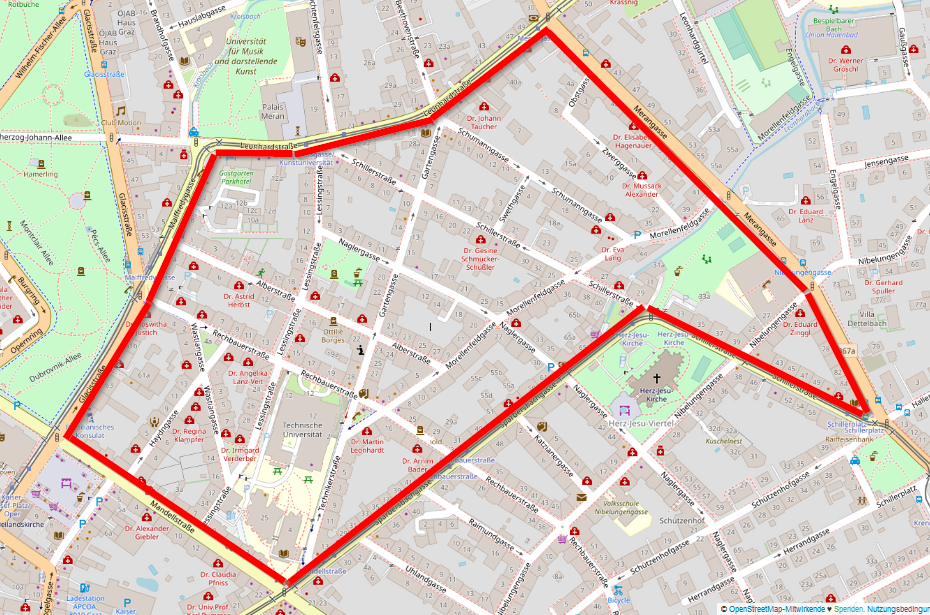
\includegraphics[width=0.8\textwidth]{main/bike/tunnel/uni/verkehrsberuhigter_bereich}
    \caption[Verkehrsberuhigkter Bereich Alte Technik]{Vorschag eines Verkehrsberuhigten Bereichs um die Alte Technik, der die Zufahrt Alte Technik noch wichtiger machen würde.}
\end{figure}

\subsection{Zufahrt Lichtenfelsgasse}
Die nächste Zufahrt befindet sich im Uni-Park ist ein wichtiger Anschluss zum \index{BG/BRG Lichtenfelsgasse} und den gesamten westlichen Bereich zwischen Leonhardstraße und Elisabethstraße.

\paragraph{Ort der Zufahrt}
\begin{figure}
    \centering
    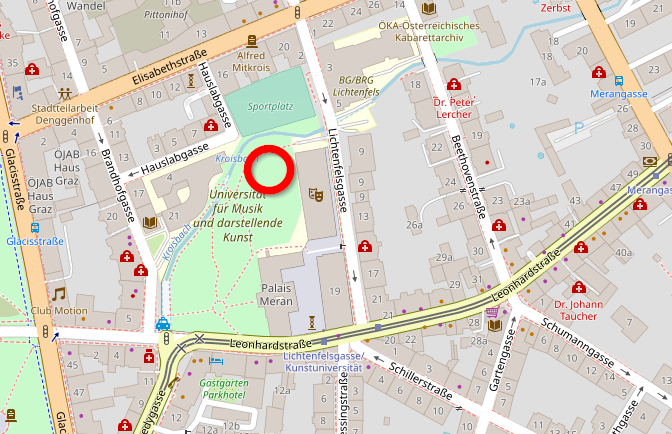
\includegraphics[width=0.8\textwidth]{main/bike/tunnel/uni/zufahrt_lichtenfelsgasse}
    \caption[Zufahrt Lichtenfelsgasse]{Zufahrt zur Lichtenfelsgasse im Uni-Park hinter der Universität für Musik und Darstellende Kunst}
\end{figure}

Die Zufahrt soll sich im Uni-Park hinter der Universität für Musik und Darstellende Kunst verbinden, da hier der einzige Platz in dieser Gegend dafür ist.

\paragraph{Anschluss}
Wichtiges Einzugsgebiet dafür sind das BG/BRG Lichtenfels, die Universität für Musik und Bildende Kunst sowie das Theater im Palais. Um einen sicheren Zugang zum Lichtenfels-Gymnasium zu ermöglichen, sollte hier überprüft werden, ob ein Übergang über die Lichtenfelsgasse angepasst werden muss. Außerdem sollte durch den Uni-Park ein Radweg mit Anschluss zur Lichtenfelsgasse und im Süden in die \index{Brandhofgasse} geplant werden.

\paragraph{Fahrradgarage}
An dieser Position sollte eine Fahrradgarage mittlerer Größe angedacht werden. Das spart einerseits Platz auf der Oberfläche, bietet aber auch genügend Abstellplätze für all jene, die zur Uni oder der Schule fahren wollen.

\paragraph{Option: Umgestaltung der Lichtenfelsgasse}
Die Hauptzufahrt zur 

\subsection{Mögliche Verlängerung nach Süden}
Von der Zufahrt Schulzentrum St. Peter aus ist eine Verlängerung nach Süden denkbar mit folgenden weiteren Zufahrten:
\begin{itemize}
    \item ORF-Park
    \item Wohnpark St. Peter
    \item Messendorf
    \item Raaba
\end{itemize}

\subsection{Mögliche Verlängerung nach Norden}
Von der Zufahrt Wirschaftskammer aus ist eine weitere Verlängerung in Richtung Norden denkbar mit folgenden weiteren Zufahrten:
\begin{itemize}
    \item Ortweinschule
\end{itemize}

Von dort aus ist das Radwegenetz auch oberirdisch gut möglich und teilweise bereits ausgebaut.